For the creation of the model, a specific architecture was chosen. That came up after many trials in the model and constantly monitoring the results of the training and evaluation processes.\\~\\
The previously mentioned architecture consists : 
\begin{itemize}
  \item At first, a Convolutional Layer is being put into the architecture that has the size of the input (50,50) with 32 filters. After that the data was passed to a max\_pooling layer, so the size can be reduced (25,25) and their characteristics get more obvious.
  \item After that we repeat the previous step for 3 more times. Firstly, the input shape is (25,25) but with 64 filters, with the same procedure as before using max\_pooling and reducing the size to (12,12). The second time the input shape is (12,12), the filters are 128 and max\_pooling reduces the size once more on to (5,5). The final time the input shape of the Convolutional Layer is (5,5) and reduced to a (2,2) after max\_pooling, keeping the filters the same as before.
  \item In the end, we add a Flatten Layer to transform the 2-dimensional array we receive after the previous layers to a vector so we can simplify the classification process. After having converted the data into a one-dimensional sequence, in order to reduce the effect of overfitting on the data with which the model is trained (not to learn specific patterns). The last stage of the network consists of two Dense Layers. The first sized 128 to reduce the data and the second, sized 2, to output the two probabilities of the objects it was trained on.
\end{itemize}
Additionally, each Convolutional Layer and the first Dense use the Rectified Linear Unit (ReLU) activation function, to activate the corresponding nodes and calculate the corresponding weights. Function's type is ReLU(x) = max(0,x), with x being the inputs and is returned when it is positive, otherwise 0 is returned. The last Dense Layer uses softmax as activitation function in order to output a probability distribution over the two possible classes and allow the CNN to make more accurate predictions.\\~\\
Furthermore, each layer has its strides set to 2. As a result the filter will move two pixels to the right at each step instead of one. This means the filter would be applied fewer times, and the resulting output (often referred to as a feature map) would be smaller. Also, same padding is used to keep the output size equal to the input size after convolution.\\~\\
The model analytically and graphicly:
\begin{figure}[H]
    \centering
    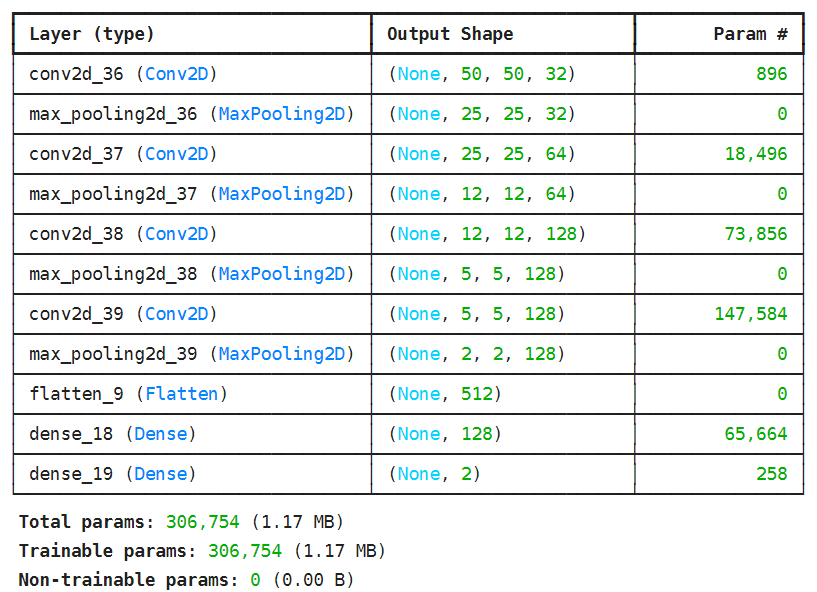
\includegraphics[width=0.8\textwidth]{Images/Screenshot 2024-04-15 184102.png}
    \caption{CNN model matrix}
    \label{fig:example}
\end{figure}
\begin{figure}[H]
    \centering
    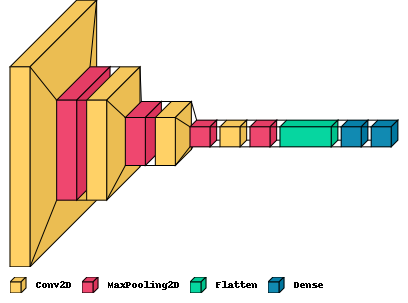
\includegraphics[width=0.8\textwidth]{Images/download.png}
    \caption{CNN model 3D Visualization}
    \label{fig:example}
\end{figure}